\section{Design af spoler}\label{sec:sec_spole_design}

\subsection{Dimensionering af spoler}

For at kunne dimensionere og designe en spole, er det væsentligt at vide hvilket formål spolen skal bruges til. Spolen har mange egenskaber, og i dette projekt vil de blive designet, så de kan bruges som sensorer. Altså en enhed der opfanger eller udsender et analogt signal. 

Som beskrevet tidligere, består systemet af i alt 3 spoler. 1 stor spole, som skal stå for at udsende et signal. Herudover 2 mindre identiske spoler, som skal opfange signalerne. For et illustrativt billede af opsætningen se afsnit **.

I den følgende tekst, vil der blive beskrevet hvilke faktorer der er blevet lagt vægt på, samt hvordan nogle af Maxwells ligninger er blevet brugt til at dimensionere de enkelte spoler. Herunder begreber som magnetfelt(B), flux$(\Phi)$, induktans(L) og elektromotorisk kraft som fremadrettet vil blive betegnet som EMF$(\xi)$. 

Først vil dimensioneringen af den store spole tages højde for, hvorefter der kigges på de 2 små spoler.
Den færdige dimensionering skal ende ud i et målbart EMF signal.

Der er som udgangspunkt taget brug af Biot-Savarts lov som ses i ligning \ref{eq:spole_biot_savart}, 


\begin{figure}[h!]
	\centering
	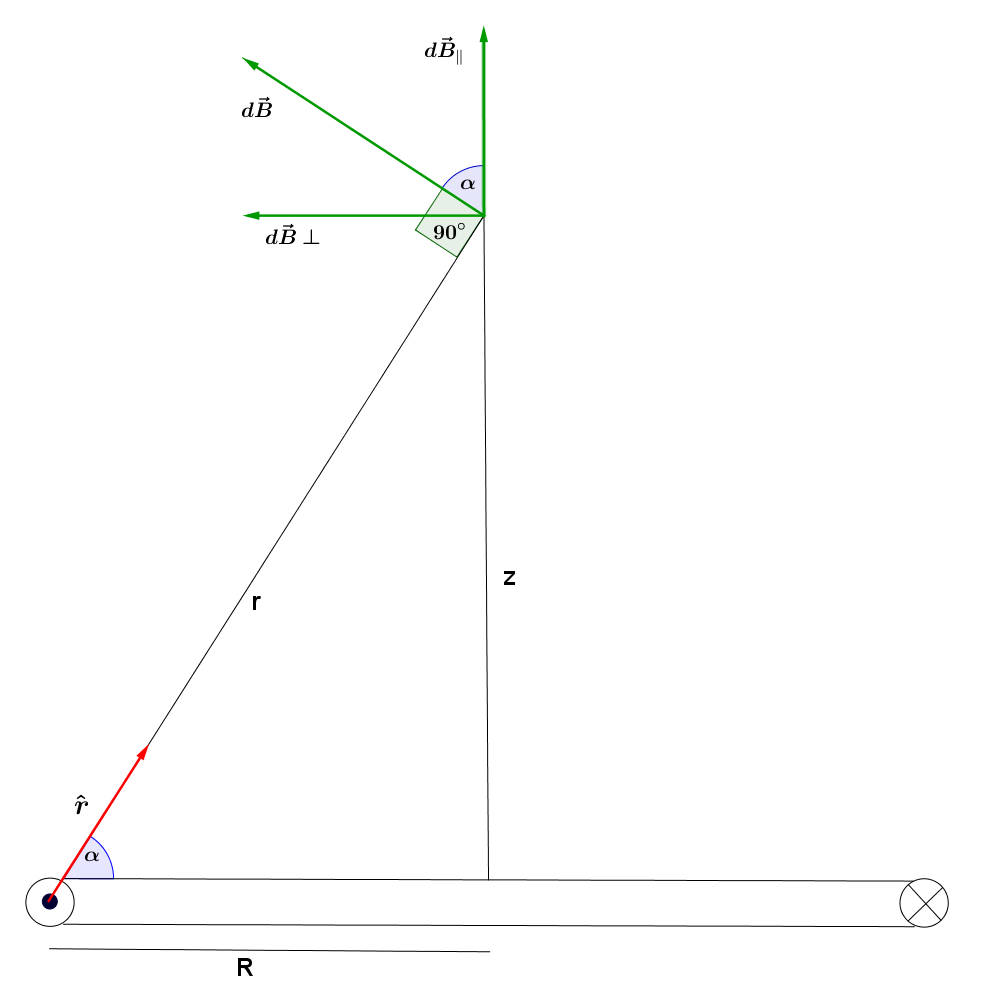
\includegraphics[width=.6\textwidth]{billeder/B_felt.png}
	\caption{Cirkulær leder med radius R}
	\label{fig:spole_fig1}
\end{figure}

På figur \ref{fig:spole_fig1} ses et tværsnit af en cirkulær leder, hvori der løber en strøm kaldet $i$. Krydset indikerer at stømmen går ind i papiret, og prikken også kaldet spidsen af en pil, indikerer at strømmen går ud af papiret. Man kan også se på denne figur, som den store spole med 1 vinding. Betragt punktet P på z aksen. I dette punkt ønskes et magnetfelts styrke bestemt, afhængig af positionen z. Som det ses er vinklen, uanset hvor på lederen man befinder sig, mellem $d\vec{s}$ og enhedsvektoren $\hat{r}$ altid $90\degree$ vinkeltret på hinanden.

Med dette kan $d\vec{B}$ feltet tegnes ind, vha. Biot-Savarts lov, eller vha. højrehåndreglen. En mere overskuelig måde at se det på er, at krydsproduktet af 2 vektorer, er en vektor der står vinkeltret på begge. 
$d\vec{B}$ kan nu deles op i 2 komposanter. En komposant $dB_\parallel$, som står parralelt på z axen og den cirkulære leder. Derudover også en komposant $dB_\perp$, som står vinkeltret på samme.

Summen af alle de vinkeltrette komposanter går ud da $d\vec{s}\times d\vec{B}_\perp=0$, og tilbage står kun de parallelle komposanter $dB_\parallel$, hvilket resulterer i:

 \begin{align}
 &B=\int dB_\parallel \label{eq:B_field}
 \end{align}

  
  
Betragt Biot-Savarts lov i ligning \ref{eq:spole_biot_savart}

\begin{align}
&d\vec{B}=\frac{\mu_0}{4\pi} \frac{i d\vec{s} \times \hat{r}}{r^2}\label{eq:spole_biot_savart}
\end{align}

Fra figur \ref{fig:spole_fig1}, kan ligning \ref{eq:spole_biot_savart} skrives om til:
\begin{align}
&dB=\frac{\mu_0}{4\pi} \frac{i ds\: sin(90\degree)}{r^2}\label{eq:spole_biot_savart2}
\end{align}
 Denne ligning giver udtryk for hvad det magnetiske felt er i en afstand $r$ fra $d\vec{s}$.
 
Ud fra figur \ref{fig:spole_fig1}, kan et udtryk for $dB_\parallel$ også vises.

 \begin{align}
 	&dB_\parallel=dB\: cos(\alpha)
 \end{align}

Hermed kan et samlet udtryk for $dB_\parallel$ gives: 

\begin{align}
&dB_\parallel=\frac{\mu_0 \:i\: cos(\alpha)\:ds}{4\:\pi\: r^2}
\end{align}

Da det er z der ønskes varieret, bliver et nyt udtryk nødt til at blive bestemt, hvor z indgår. Betragt figur \ref{fig:spole_fig1} igen. Her ses, at $r$ og vinklen $\alpha$, er relateret til hinanden, og ved hjælp at Phytagoras, kan disse 2 udtryk findes:


\begin{align}
&r=\sqrt{R^2+z^2}
\end{align}

og

\begin{align}
&cos(\alpha)=\frac{R}{r}=\frac{R}{\sqrt{R^2+z^2}}
\end{align}

Da $i, R$ og $z$ alle har samme værdi for alle $ds$ hele vejen rundt i den cirklære leder, kan man vha. integration summere op, på samme måde som deffineret i ligning \ref{eq:B_field}, og der fås dermed et udtryk for B:



\begin{align}
&B=\frac{\mu_0 \: i \: R}{4\pi(R^2+z^2)^\frac{3}{2}}\int ds
\end{align}

Grænseværdierne for $\int ds$ er den cirkulære leders omkreds.

\begin{align}
&\int\limits_{0}^{2\pi R} ds = 2\pi R
\end{align}

Et endeligt udtryk for magnetfeltet $B(z)$ gives i ligning \ref{eq:Bz_field}.

\begin{align}
	&B(z)=\frac{\mu_0 \: i \: R^2}{2(R^2+z^2)^\frac{3}{2}} \label{eq:Bz_field}
\end{align}


Da dette udtryk kun er gældende for en cirkulær leder, altså en luftspole med 1 vinding, skal et nyt udtryk bestemmes. Dette udtryk tager udgangspunkt i ligning \ref{eq:Bz_field}, som blev udledt før.

\begin{figure}[h!]
	\centering
	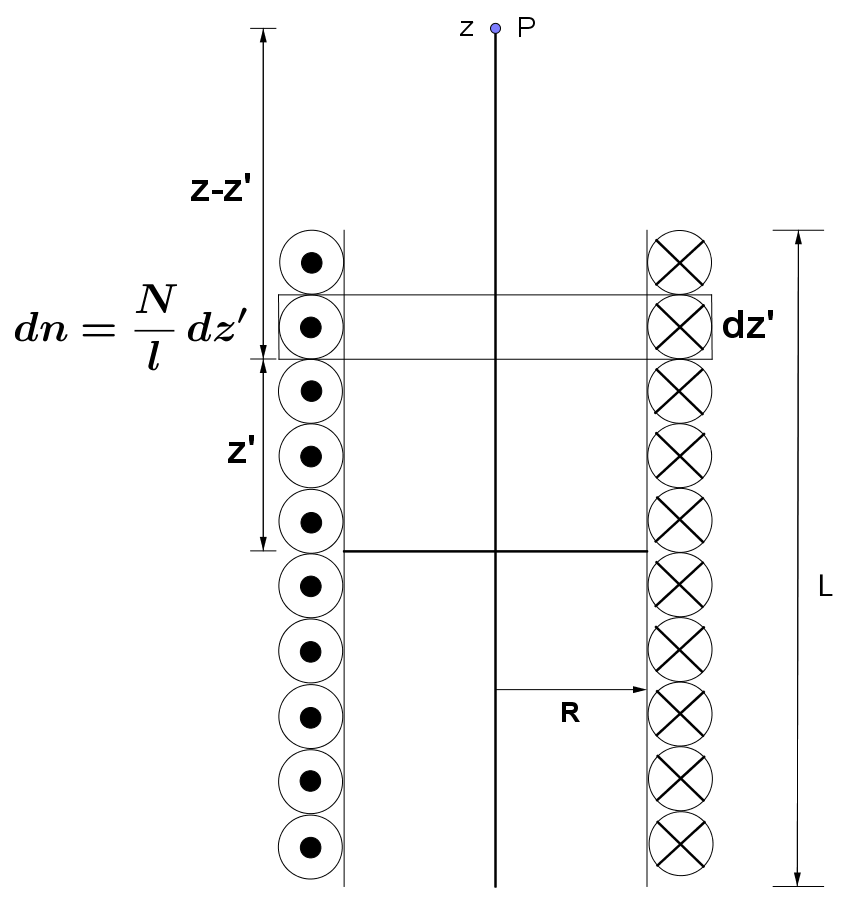
\includegraphics[width=.5\textwidth]{billeder/B_felt2.png}
	\caption{Solenoid med radius R}
	\label{fig:spole_fig2}
\end{figure}

Formlen for B feltet i en uendelig lang solenoid er givet ved:

\begin{align}
	&B=\mu ni
\end{align}

Hvor $n$ er antal vindinger pr. længde:


\begin{align}
	&n=\frac{N}{L}
\end{align}

I dette udtryk er B feltet centreret i midten af den uendelig lange solenoide.

Da solenoidestørrelsen er bestemt, og ikke uendelig lang, samt $B$ feltet ligger uden for solenoidens yderkant, skal en ny ligning af $B$ feltet bestemmes.
Det antages at $B$ feltet er homogent omkring hele fladen, og ikke kun i det punkt der bestemmes.


Betragt figur \ref{fig:spole_fig2}. Her ses tværsnittet af en solenoide, med z aksen i centrum. Det ønskede $B$ felt skal bestemmes i punktet $P$.

Det ses at størrelsen af $n$ er proportional med tykkelsen $dz'$:

\begin{align}
	&dn=\frac{N}{L} dz'
\end{align}



Ud fra ligning \ref{eq:Bz_field}, kan $dB_z$ udtrykkes ved: 

\begin{align}
	&dB(z)=\frac{\mu_0 \: i \: R^2}{2(R^2+(z-z')^2)^\frac{3}{2}}dn=\frac{\mu_0 \: N \: i \: R^2}{2L(R^2+(z-z')^2)^\frac{3}{2}}dz'
\end{align}

Ved at integrerer over hele længden på solenoiden fås:

\begin{align}
	&B(z)=\int\limits_{-\frac{L}{2}}^{\frac{L}{2}}\frac{\mu_0 \: N \: i \: R^2}{2L(R^2+(z-z')^2)^\frac{3}{2}}dz'
\end{align}

Og et endeligt udtryk:
\begin{align}
	&B(z)= \frac{\mu_0 \: i \: R^2 \: N}{2L}\bigg(\frac{\frac{L}{2}-z}{\sqrt{(z-\frac{L}{2})^2+R^2}}+\frac{\frac{L}{2}+z}{\sqrt{(z+\frac{L}{2})^2+R^2}}\bigg)
\end{align}


%
%\begin{align}
%	&di=inz'
%\end{align}
%
%\begin{align}
%	&n=\frac{N}{L}
%\end{align}
%
%\begin{align}
%	&d\vec{B}=\frac{\mu_0 R^2}{2[(z-z')^2+R^2]^\frac{3}{2}}di = \frac{\mu_0 R^2 i n dz'}{2[(z-z')^2+R^2]^\frac{3}{2}}
%\end{align}
%
%
%B felt i et givet punkt P centreret ud fra z aksen, med funktion af z er dermed givet ved:
%\begin{align}
%	&B(z)=\frac{\mu_0 n R^2 i}{2}\int\limits_{0}^{2\pi}\frac{1}{2[(z-z')^2+R^2]^\frac{3}{2}}dz'
%\end{align}
%
%\begin{align}
%	&B(z)=\frac{\mu_0 n i}{2}\bigg[\frac{\frac{L}{2}-z}{\sqrt{(\frac{z-L}{2})^2+R^2}}+\frac{\frac{L}{2}+z}{\sqrt{(\frac{z+L}{2})^2+R^2}}\bigg]
%\end{align}

\subsection{3D design/fysisk design af spolehus}
\begin{itemize}
	\item Inventor
	\item PnP system
	\item Huller til vindingsmaskine
	\item Clamp
\end{itemize}
Spolerne er designet således at når den store spole er i nul (i midten) overlapper den de mindre spoler så de er dækket præcist 50\percent. Når den store spole så er i sin fulde udslagsvinkel er hhv. den ene mindre spole dækket helt, hvor den anden slet ikke er dækket. \\

Illustration af forklaring her...

\emph{Introduktion til emnet i kapitlet skrives her}
\begin {itemize}
\item Udnytter forudborede huller
\item Batteri"slots"
\item Standoff mounts til print

\item Udgangssignalet på spolen skal filtreres og ensrettes
\item Aktivt båndpas filter, fordele vs. passivt
\item Indsnævring af frekvens
\item Ensretteren/konvertering til DC
\item Regulator-venligt signal. 

\item 555 generator
\item Firkantsignal
\item Opsætning 
\item Modstandsbestemmelse
\end {itemize}
